

\tikzset{every picture/.style={line width=0.75pt}} %set default line width to 0.75pt        

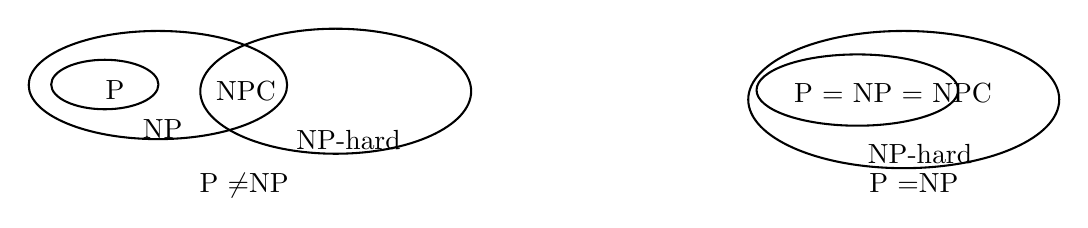
\begin{tikzpicture}[x=0.5pt,y=0.5pt,yscale=-1,xscale=1]
%uncomment if require: \path (0,124); %set diagram left start at 0, and has height of 124

%Shape: Ellipse [id:dp5973445750134718] 
\draw   (2.75,41.92) .. controls (2.75,20.33) and (44.56,2.83) .. (96.13,2.83) .. controls (147.69,2.83) and (189.5,20.33) .. (189.5,41.92) .. controls (189.5,63.5) and (147.69,81) .. (96.13,81) .. controls (44.56,81) and (2.75,63.5) .. (2.75,41.92) -- cycle ;
%Shape: Ellipse [id:dp8841818331933643] 
\draw   (19,41.54) .. controls (19,31.66) and (36.35,23.66) .. (57.75,23.66) .. controls (79.15,23.66) and (96.5,31.66) .. (96.5,41.54) .. controls (96.5,51.42) and (79.15,59.42) .. (57.75,59.42) .. controls (36.35,59.42) and (19,51.42) .. (19,41.54) -- cycle ;
%Shape: Ellipse [id:dp3401453478358991] 
\draw   (126.75,46.39) .. controls (126.75,21.44) and (170.57,1.21) .. (224.63,1.21) .. controls (278.68,1.21) and (322.5,21.44) .. (322.5,46.39) .. controls (322.5,71.33) and (278.68,91.56) .. (224.63,91.56) .. controls (170.57,91.56) and (126.75,71.33) .. (126.75,46.39) -- cycle ;
%Shape: Ellipse [id:dp5090440012854042] 
\draw   (528.75,45.55) .. controls (528.75,31.32) and (561.38,19.79) .. (601.63,19.79) .. controls (641.87,19.79) and (674.5,31.32) .. (674.5,45.55) .. controls (674.5,59.78) and (641.87,71.31) .. (601.63,71.31) .. controls (561.38,71.31) and (528.75,59.78) .. (528.75,45.55) -- cycle ;
%Shape: Ellipse [id:dp5250684881928416] 
\draw   (522.75,52.41) .. controls (522.75,25.03) and (573.06,2.83) .. (635.13,2.83) .. controls (697.19,2.83) and (747.5,25.03) .. (747.5,52.41) .. controls (747.5,79.8) and (697.19,102) .. (635.13,102) .. controls (573.06,102) and (522.75,79.8) .. (522.75,52.41) -- cycle ;

% Text Node
\draw (553.59,38.68) node [anchor=north west][inner sep=0.75pt]   [align=left] {P = NP = NPC};
% Text Node
\draw (608,103.5) node [anchor=north west][inner sep=0.75pt]   [align=left] {P $\displaystyle =$NP};
% Text Node
\draw (607,82.6) node [anchor=north west][inner sep=0.75pt]   [align=left] {NP-hard};
% Text Node
\draw (56,36.56) node [anchor=north west][inner sep=0.75pt]   [align=left] {P};
% Text Node
\draw (136,37.37) node [anchor=north west][inner sep=0.75pt]   [align=left] {NPC};
% Text Node
\draw (83,64.83) node [anchor=north west][inner sep=0.75pt]   [align=left] {NP};
% Text Node
\draw (124,103.5) node [anchor=north west][inner sep=0.75pt]   [align=left] {P $\displaystyle \neq $NP};
% Text Node
\draw (194,72.1) node [anchor=north west][inner sep=0.75pt]   [align=left] {NP-hard};


\end{tikzpicture}

